\subsection{How does NetML work in Fault Localization?}
NetML contains two sets of latent parameters (i.e., bug reports and methods). The incorporation of the latent parameters provides NetML with a higher freedom to capture the relationship of different bug reports and methods more accurately. Moreover, NetML also employs the network Lasso regularization in its learning procedure, which imposes similar bug reports (and methods) to have similar latent parameters. Outputs of our NetML include the latent parameters of bug reports ($\mathbf{U}$) and methods ($\mathbf{V}$). Please refer to Section~\ref{sec:approach} for more details about NetML. 

Based on the latent parameters of bug reports (or methods), we apply cosine similarity~\cite{Salton:1975:VSM:361219.361220} to estimate how these bug reports are similar in latent space. Then we present some qualitative examples to illustrate the poor/good performance of NetML compared to other techniques. %More specifically, we show four case samples as follows:
%\begin{itemize}
%	\item A high cosine similar score of latent parameters between two bug reports. 
%	\item A low cosine similar score of latent parameters between two bug reports. 
%	\item A high cosine similar score of latent parameters between two methods. 
%	\item A low cosine similar score of latent parameters between two methods. 	
%\end{itemize}

\subsubsection{Case Examples of NetML: Good Results in Detecting Bugs}
\label{sec:case_good}
We introduce two examples defect to illustrate why NetML performs well in fault localization problem. We consider two bugs (i.e., Bug 720 and Bug 857) in project Lang. Bug 720 issues an ``outputs wrong results, when an input contains characters in \textit{Supplementary Planes}'' whereas Bug 857 contains ``\textit{StringIndexOutOfBoundsException}'' error. These two bugs ultimately reside in the \texttt{translate} method in the \texttt{CharSequenceTranslator.java} program. To find this method, based on the report, the developer could apply IR-based or spectrum-based bug localization techniques to generate a ranked list of methods. The list could then be inspected, in order, until the root cause of the bug is localized. Figure~\ref{fig:bug_high_crop} shows the description of two bugs (i.e., Bug 720 and Bug 857) in project Lang, which contains 5,528 methods. AML and SAVANT assign Bug 857 a high priority, i.e., localizing the \texttt{translate} method in the top 10 of the produced list. However, AML and SAVANT assign Bug 720 a low priority, i.e., localizing the \texttt{translate} method in the top 100 of the produced list. None of eight state-of-the-art spectrum fault localization techniques (i.e., OCHIAI, DSTAR, PROMESIR, DIT$^\text{A}$, DIT$^\text{B}$, LR$^\text{A}$, LR$^\text{B}$, and MULTRIC) localize the \texttt{translate} method within the top 10 of the produced list in both Bug 720 and Bug 857. The two best performance of spectrum fault localization approaches for this defect (i.e., OCHIAI and DSTAR) assigns the highest suspiciousness score to the faulty method; however, there are more than 100 methods sharing this score. Existing spectrum-fault localization approaches present limited utility for the developer in this case. 

On the other hand, NetML assigns Bug 720 and Bug 857 a high priority, which successfully localizes the faulty method (i.e., \texttt{translate}) within the top 10 of the produced list. Typically, we see that both NetML and AML assign Bug 857 a high priority. However, we assume that NetML takes advantages of the latent parameters of the two similar bug reports, and enforce them to have similar latent parameters. To explain our assumption, we apply a \textit{Vector Space Model} (VSM) to estimate the similarity between Bug 720 and Bug 857 at this space. We represent each bug report as vectors of weights; each weight corresponds a term. We evaluate the value of each weight by applying TF-IDF~\cite{Ramos1999} and estimate cosine similarity of Bug 857 with the remaining bug reports. We found that Bug 720 is ranked at position \textit{\#}39. We took the latent parameters of bug reports, which are the matrix $\mathbf{U}$ (please refer to Algorithm~\ref{alg:network_lasso}). We again estimate the cosine similarity of Bug 857 with the remaining bug reports in a latent space. In this case, Bug 720 is ranked at position \textit{\#}5. It shows that these two bugs are actually very close in the latent space. Indeed, these two bugs share the same \texttt{translate} method and  \texttt{CharSequenceTranslator} program, and these two bugs should be similar. AML only assumes that bug reports are independent, leading to failing to assign Bug 720 a high priority. On the other hand, NetML tries to enforce the similar bug reports to have similar latent parameters, leading to successfully to assign Bug 720 a high priority. 

Figure~\ref{fig:method_high_crop} presents the description of Bug 93 in project Time, which contains 4,181 methods. Bug 93 issues an error when ``weekyear has a null range duration type''. The bug resides in the \texttt{partial} and \texttt{compareTo} methods of the \texttt{Partial.java} and \texttt{UnsupportedDurationField.java} programs respectively. AML localizes the \texttt{partial} method in the top 5 of the produced list, however AML ranks the \texttt{compareTo} method at position \textit{\#}35. SAVANT also restricts the \texttt{partial} method in the top 10, and it ranks \texttt{compareTo} method at position \textit{\#}87. The spectrum fault localization techniques rank these two methods outside the top 100 of the produced list, which assigns this bug a low priority. NetML localizes the \texttt{partial} and \texttt{compareTo} methods at the rank \textit{\#}3 and \textit{\#}10 of the produced list respectively, which assigns Bug 93 a high priority. Similar to bug reports, we again calculate the similarity between two methods at the low space (vector space) and latent space. We collected the latent parameters of methods which are the matrix $\mathbf{V}$ (please refer to Algorithm~\ref{alg:network_lasso}). By applying VSM, we estimate cosine similarity of \texttt{partial} method with the remaining methods. We found that \texttt{compareTo} method is ranked at position \textit{\#}981. However, \texttt{compareTo} method is ranked at position \textit{\#}32 in the latent space. By looking at the content of these two methods, we see that they share the same parameter \texttt{DurationField} and \texttt{compareTo}, hence these methods should be close. AML assumes that methods are independent, leading to failing to localize the faulty \texttt{compareTo} method. NetML enforces the similar methods to have highly similar latent parameters, leading to successfully to localize \texttt{compareTo} method at rank \textit{\#}10. 

\subsubsection{Case Examples of NetML: Poor Results in Detecting Bugs}
\label{sec:case_bad}
We first introduce two examples defect to show why NetML achieves poor performance in fault localization problem. We consider Bug 617 and Bug 710 in project Lang. Bug 617 contains an error of ``process UTF-16 supplementary characters'' whereas Bug 710 has ``StringIndexOutOfBoundsException'' when we call a special string. These two bugs are related the \texttt{escapeXML} method in the \texttt{StringEscapeUtils.java} program. Figure~\ref{fig:bug_low} presents the details of these two bugs. NetML, AML, and SAVANT assign Bug 617 a high priority, however they fail to localize the faulty \texttt{escapeXML} method for Bug 710. Intuitively, \texttt{escapeXML} method and \texttt{StringEscapeUtils} program were clearly mentioned in Bug 617, hence should be easily captured by applying IR-based localization technique. OCHIAI and DSTAR estimate the highest suspiciousness score to the \texttt{escapeXML} method for both Bug 617 and Bug 710; however, we have around 50 methods sharing this score. The remaining baselines (i.e., PROMESIR, DIT$^\text{A}$, DIT$^\text{B}$, LR$^\text{A}$, LR$^\text{B}$, and MULTRIC) fail to localize these two bugs in a high priority. By reading the content of Bug 710, we see that this bug does not contain any information related to \texttt{escapeXML} method. Moreover, the suspiciousness score of the faulty method, which is calculated by using spectrum-fault localization, often shares with another methods. For these reasons, it is a challenge to assign a high priority for Bug 710. Similar to Section~\ref{sec:case_good}, we calculate the similarity score between these two bugs at low and latent spaces. We estimate the similarity of Bug 617 with the remaining bug reports. We found that Bug 710 is ranked at position \textit{\#}55 and \textit{\#}48 in the low level space and latent space, respectively. It shows that these two bugs are independently, and hence NetML fails to localize the faulty method for bug 710.

Figure~\ref{fig:method_low} shows the descriptions of Bug 18 in project Time. Bug 18 issues an null pointer exception when ``a DateTimeZone is build with duplicate-named''. The bug contains two faulty methods, i.e., \texttt{RuleSet} and \texttt{DateTimeOfYear}, in \texttt{ZoneInfoCompiler.java} program. NetML, AML, and SAVANT localizes the \texttt{RuleSet} method in the top 10 of produced list, however these techniques rank \texttt{DateTimeOfYear} method outside the top 50. OCHIAI and DSTAR rank these methods at the highest suspiciousness score, however we have 42 methods sharing this score. The other baselines fail to localize the two faulty methods within the top 50 of the produced list. We again estimate the similarity score between the two methods at a low level space and latent space. We calculate the similarity of method \texttt{RuleSet} against the remaining methods in Time. Method \texttt{DateTimeOfYear} is ranked at position \textit{\#} 2,678 and \textit{\#}2,468 in the low level space and latent space, respectively. It shows that these two methods independent with each other, hence NetML is unable to localize method \texttt{DateTimeOfYear}.

%\begin{figure*}[!t]
%	\centering
%	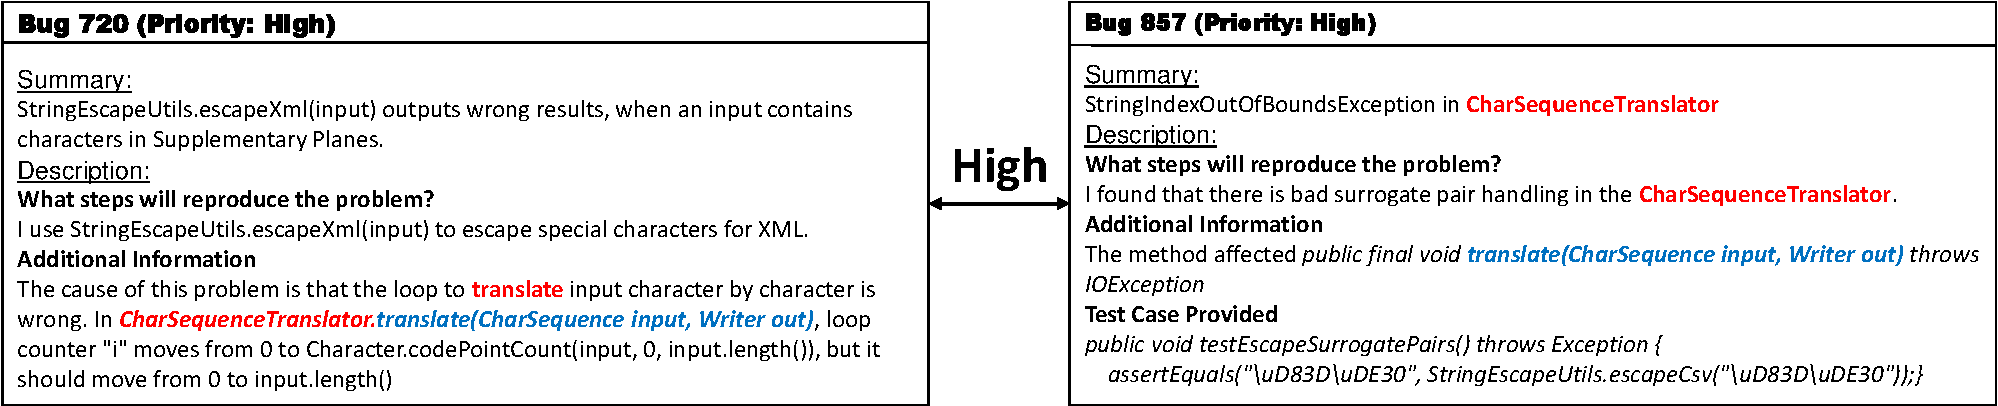
\includegraphics[width=\textwidth]{bug_high_crop}
%	\caption{The proposed NetML framework}
%	\label{fig:bug_high_crop}
%\end{figure*}

\begin{figure*}
	\centering
	\begin{subfigure}[b]{\textwidth}
		\centering
		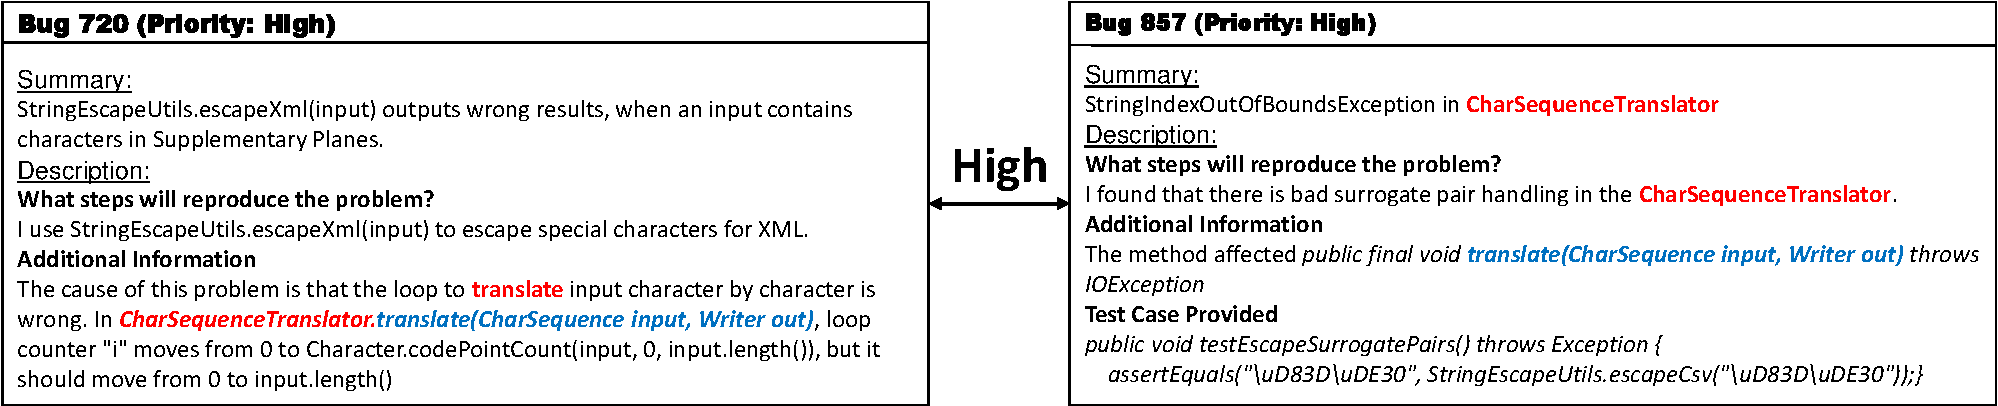
\includegraphics[width=\textwidth]{bug_high_crop}
		\caption[]%
		{{\small A case example which NetML achieves a good results. Two bug reports are highly similar at latent space.}}    
		\label{fig:bug_high_crop}
	\end{subfigure}
	\centering
	\begin{subfigure}[b]{\textwidth}  
		\centering 
		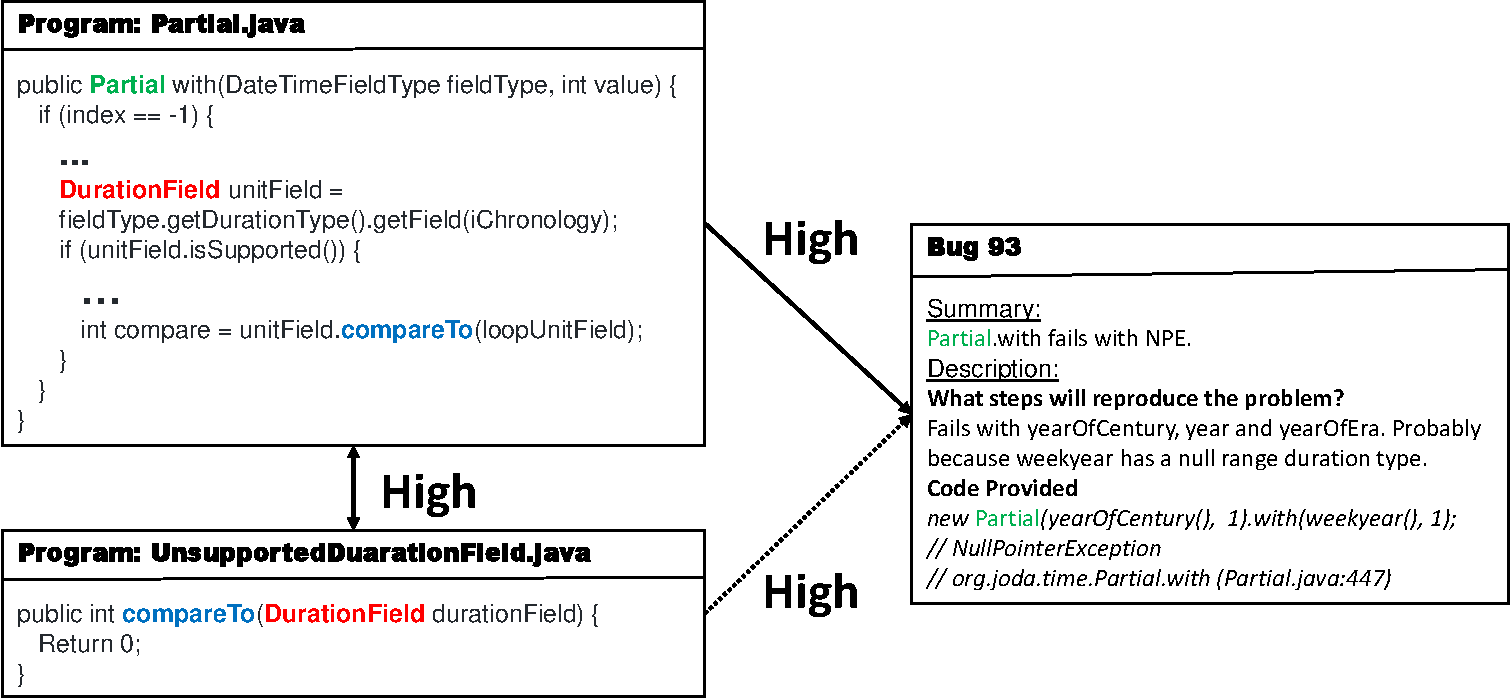
\includegraphics[width=\textwidth]{method_high_crop.pdf}
		\caption[]%
		{{\small A case example which NetML achieves a good results. Two methods are highly similar at latent space.}}    
		\label{fig:method_high_crop}
	\end{subfigure}
	\caption[]
	{\small A list of case examples to illustrate why NetML achieves good performance.}
\label{fig:case_good_example}

\end{figure*}
\begin{figure*}
	\centering
	\begin{subfigure}[b]{\textwidth}
		\centering
		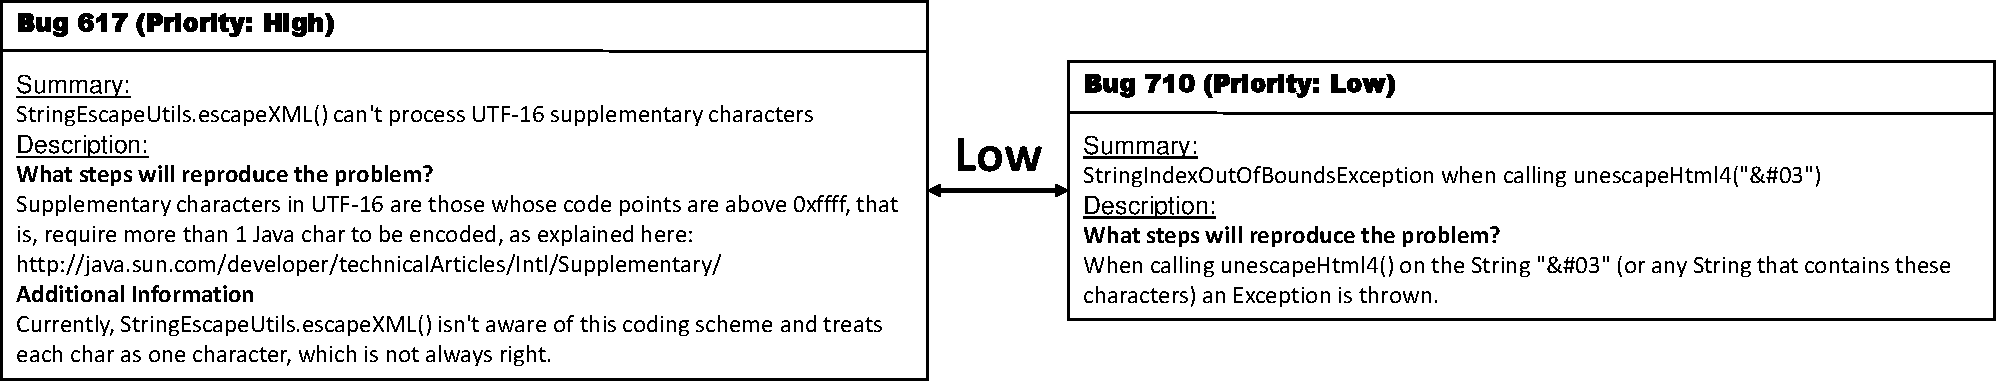
\includegraphics[width=\textwidth]{bug_low}
		\caption[]%
		{{\small A case example which NetML achieves a bad results. Two bug reports has a low similar at latent space.}}    
		\label{fig:bug_low}
	\end{subfigure}
	\centering
	\begin{subfigure}[b]{\textwidth}  
		\centering 
		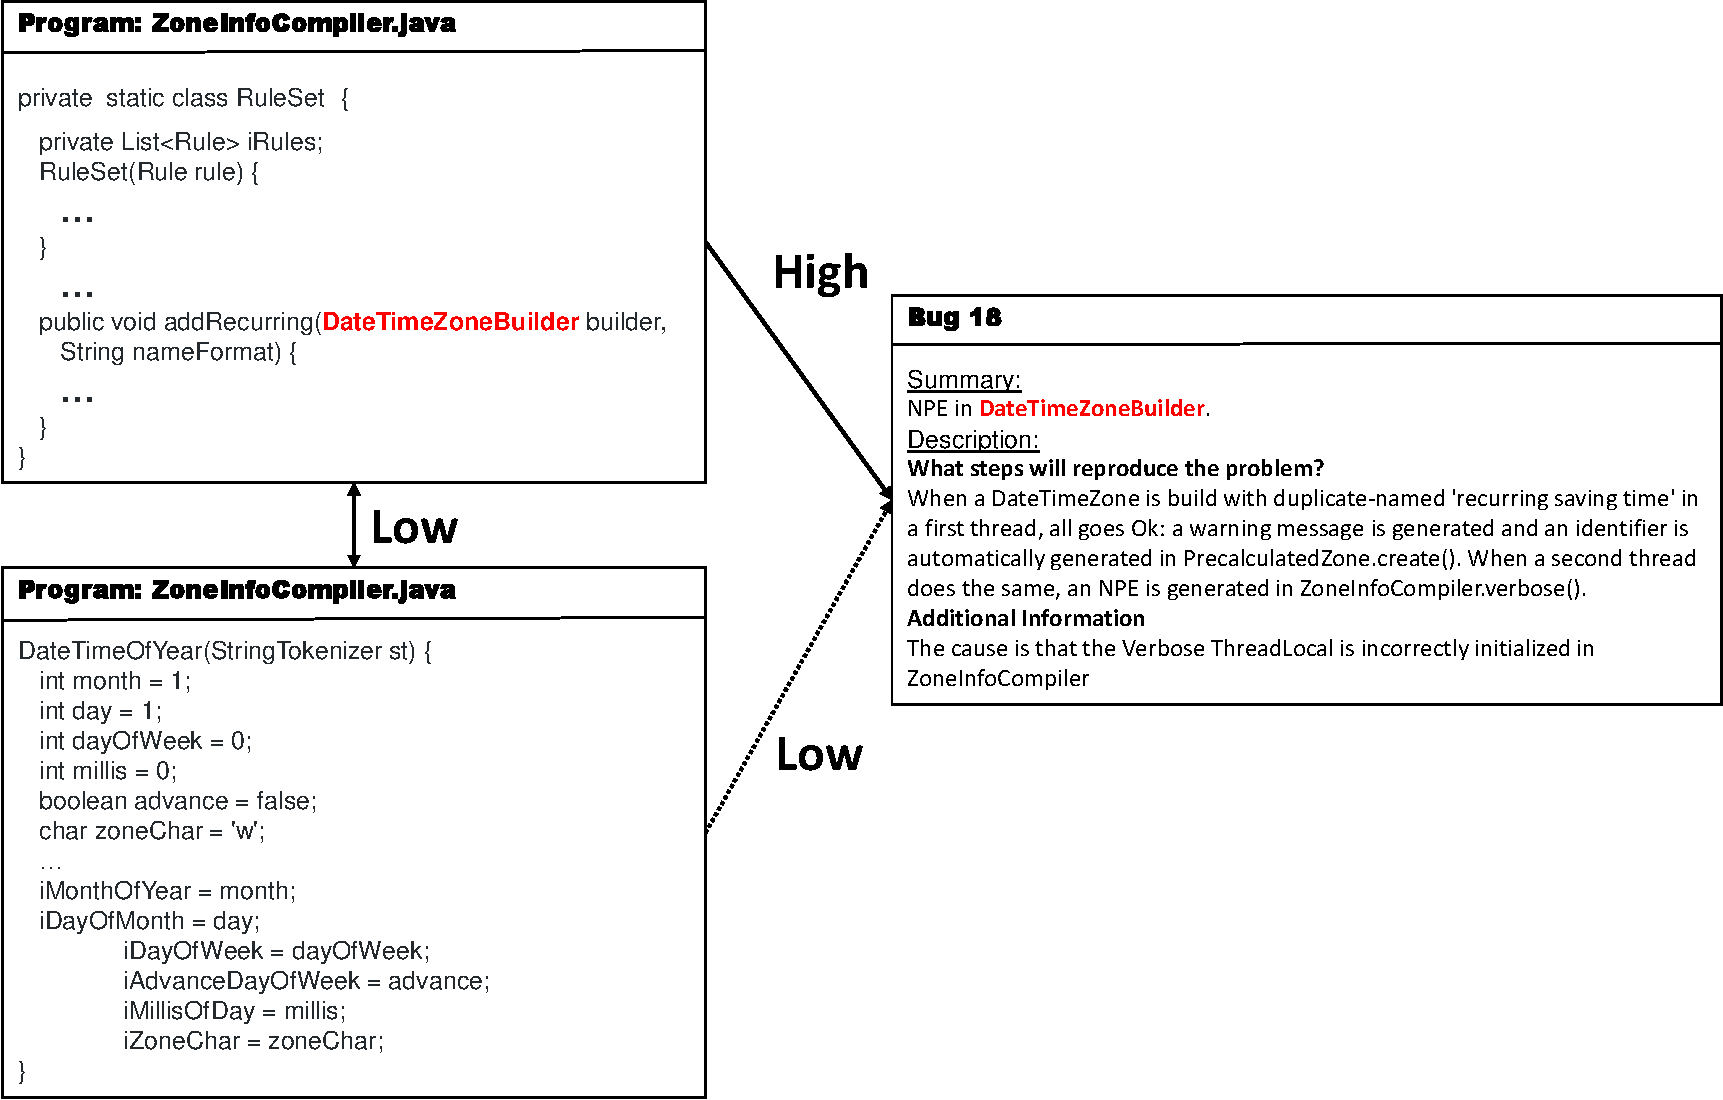
\includegraphics[width=\textwidth]{method_low_crop.pdf}
		\caption[]%
		{{\small A case example which NetML achieves a bad results. Two methods has a low similar at latent space.}}    
		\label{fig:method_low}
	\end{subfigure}
	\caption[]
	{\small A list of bad case examples to illustrate why NetML achievespoor performance.} 
	\label{fig:case_bad_example}
\end{figure*}
